\documentclass{article}
\usepackage{tabu}
\usepackage{qtree}
\usepackage{comment}
\usepackage{graphicx}
\begin{document}

\title{CS 260: Homework 5}
\author{Daniel Lopez}
\maketitle

\date{4 August 2017}

\section{1}
\begin{center}
	\begin{comment}
	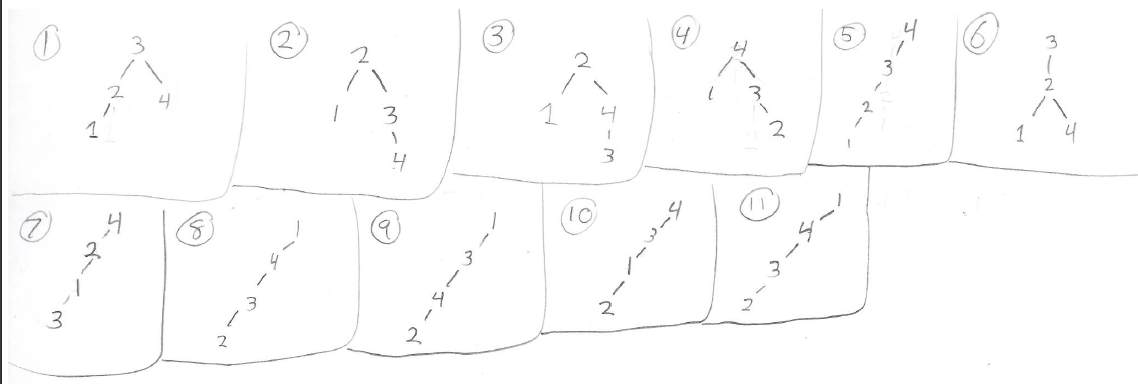
\includegraphics[scale=0.5]{Prob1.jpg}
	\end{comment}
\end{center}

\section{2}
\Tree[.7 [.2 [.0 [.1 ]]
				 [.5 [.6 ]]]
			[.9 [.8 ]]]

\section{3}
\begin{center}
	\begin{comment}
	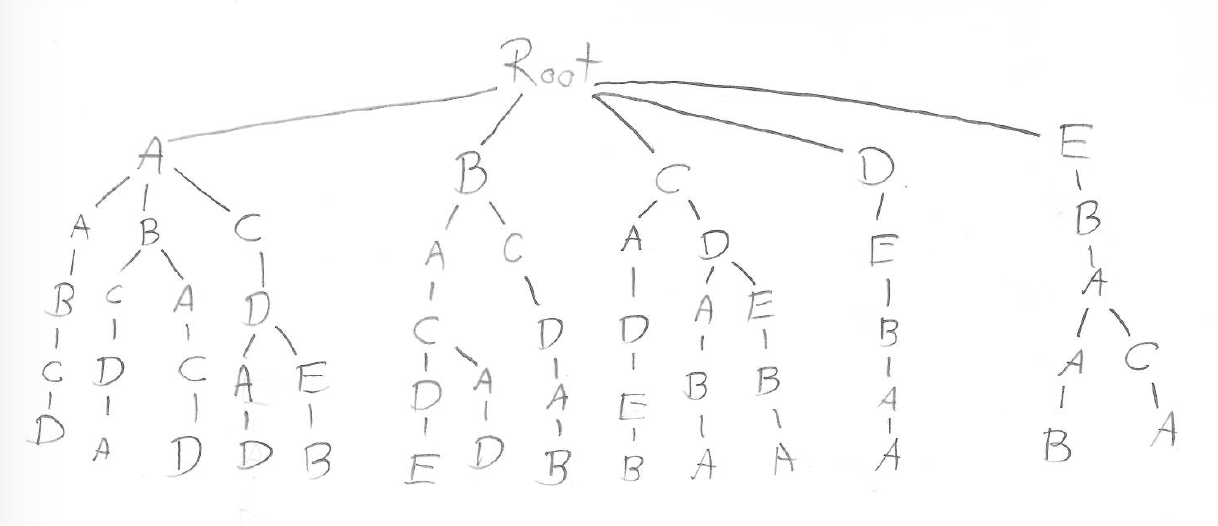
\includegraphics[scale=0.5]{Prob3.jpg}
	\end{comment}
\end{center}
\begin{comment}
Tree runs off of page. The drawing is theresulting tree from code below and is included as a graphic.
\Tree[.Root [.A [.A \textit{B}
						  \textit{C}
						  \textit{D} ]
					 [.B [.C \textit{D}
						  		\textit{A} ]
					 	  [.A \textit{C}
						  		\textit{D} ]]
					 [.C \textit{D} [.A \textit{D} ]
					 	  		[.E \textit{B} ]]]
			 [.B \textit{A} 
				  [.C [.D \textit{E} ]
						[.A \textit{D} ]]
			 	  [.C \textit{D}
						\textit{A}
						\textit{B} ]]
			[.C [.A \textit{D}
					  \textit{E}
					  \textit{B} ]
				 [.D [.A \textit{B}
					  		\textit{A} ]
					  [.E \textit{E}
							\textit{B}
							\textit{A} ]]]
			[.D \textit{E}
				 \textit{B}
				 \textit{A}
				 \textit{A} ]
			[.E \textit{B}
				 [.A \textit{A}
					  \textit{B} ]
				 [.C \textit{A} ]]]
\end{comment}
\section{4}
\Tree[.(5,7) [.(3,4) [.(0,2) [.0 ] [.1 ] [.2 ]] [.(3,-) [.3 ]] [.(4,-) [.4 ]]]
	  			 [.(6,7) [.(5,-) [.5 ]] [.(6,-) [.6 ]] [.(7,-) [.7 ] [.8 ] [.9 ] ]]]
\end{document}
